\section{Experiment Design}
Any \textbf{measurement}, without \textbf{knowledge of the uncertainty}, is \textbf{meaningless}.
Here, "meaningless" means a measurement lacks reliability if its uncertainty is unknown.
Without knowing its precision or accuracy, the value cannot be trusted or interpreted and may be \textbf{misleading}.

Experimental measurements are essential to understand system behavior, allowing us to:
\begin{itemize}
    \item Decide to \textbf{ship or not} our system;
    \item \textbf{Identify} possible improvement points for next iterations;
    \item \textbf{Communicate} system behavior to others stakeholders or colleagues.
\end{itemize}
Our final goal is to estimate how well our system performs for certain properties of interest, 
under some conditions, and for a specific population of inputs.

For AI systems, we refer to experiment rather than test or evaluation since each time we work on a “sample” of the data.
The results depend not only on the dataset, but also the specific version of the system, 
the workflow, previous experiments and randomness in the LLM.

\subsection{Basic, Probabilities and Random Variables}
Before diving into the design of experiments, we need to understand some basic concepts of probability and random variables, 
which are essential to properly design and analyze experiments.

\subsubsection{Definition of Probability}
From a general perspective, probability is a number between 0 and 1 to which we assign a meaning.
A frequentist may define probability as a \textit{proportion} 
\[\frac{\text{\#event occurrences}}{\text{\#repetitions}}\]
as the number of repetitions tends to infinity.

However, this approach cannot work in our case, since we cannot repeat experiments infinitely, and we cannot experiment always in the same conditions.
More generally, we define probability as "\textit{A belief/likelihood of an event occurring}" or  "\textit{a belief on the distribution of a random variable}".

More formally we define:
\begin{itemize}
    \item \textbf{Sample Space (S)}: The set of all possible outcomes of an experiment.
    Taking as an example an AI Judge, rating the output of our AI System on a scale from 1 to 5, the sample space would be $S = \{1, 2, 3, 4, 5\}$.
    \item \textbf{Event (E)}: An event is a subset of the sample space that satisfies some conditions.
    For example, the event $E$ that the judge rates the output as "good" could be defined as $E = \{4, 5\}$.
    \item \textbf{Probability (P(E))}: A measure of the likelihood of an event occurring, defined on the sample space.
\end{itemize}

\subsubsection{Frequentist vs Bayesian Interpretation of Probability}
There are different interpretations of probability, and the two most common ones are the frequentist and Bayesian interpretations.

\paragraph{Frequentist Interpretation} 
The frequentist interpretation defines probability as the long-run relative frequency of an event occurring in repeated trials of an experiment.
\[ P(E) = \lim_{n \to \infty} \frac{n(E)}{n} \]
where $n(E)$ is the number of times event $E$ occurs in $n$ trials.

Given the previous example of the AI Judge, if we run the experiment 200 times and the judge rates the output as "good" 140 times, 
we would estimate the probability of event $E$ as $P(E) = \frac{140}{200} = 0.70$.

\paragraph{Bayesian Interpretation}
The Bayesian interpretation defines probability as a degree of belief or confidence in the occurrence of an event, which can be updated as new evidence is obtained.
\[ P(E) = P(E | I) = belief\]
where $I$ is our prior information about the event, and $P(E | I)$ represents our belief about the probability of event $E$ given that information.

This can be seen as an estimation of the frequentist probability, where the belief is updated as new evidence is obtained, following Bayes' theorem.

\subsubsection{Axioms of Probability}
We can define the set of axioms that any probability measure must satisfy:
\begin{itemize}
    \item \textbf{Non-negativity}: $P(E) \geq 0 \quad \forall E \in S$
    \item \textbf{Normalization}: $P(S) = 1$
    \item \textbf{Complement Rule}: $P(E') = 1 - P(E)$, where $E'$ is the complement of $E$.
\end{itemize}

\paragraph{Mutual Exclusion}
We say that an event $E$ is \textbf{mutually exclusive} with another event $F$ if they cannot occur simultaneously. 
In this case, we have that:
\begin{equation}
    P(E \cup F) = P(E) + P(F)
\end{equation}
Meaning that the probability of either event $E$ or event $F$ occurring is the sum of their individual probabilities, since they cannot happen at the same time.
This is the simplest case, and can be extended to more than two events.

\paragraph{Equally likely Events}
In the case where all outcomes are \textbf{equally likely}, we can calculate the probability of an event $E$ as:
\begin{equation}
    P(E) = \frac{|E|}{|S|}
\end{equation}
Where $|E|$ is the number of outcomes in event $E$, and $|S|$ is the total number of outcomes in the sample space.

However, in many cases, especially in AI systems, we cannot assume that all outcomes are equally likely.
For example, the likelihood of an LLM generating a specific output may not be the same for all possible outputs.
This requires us to run experiments to estimate the probabilities of different outcomes, and to understand the distribution of the outputs generated by the system.

\subsection{Random Variables}
We define a \textbf{random variable} as a function that maps each outcome of an experiment to a real number, capturing uncertainty.
Assigning a value to a random variable defines an event, and we can describe its behavior with a probability distribution.

For example, in a coin toss, let $X$ be 1 for heads and 0 for tails.
This is a \textbf{binary random variable} since it takes two values.
If both outcomes are equally likely, the probability distribution is:
\begin{equation}
    P(X=1) = 0.5, \quad P(X=0) = 0.5
\end{equation}

We can do the same for an AI Judge. Starting from the sample space $S = \{1, 2, 3, 4, 5\}$, we can transform it into a binary random variable $X$ 
where $X=1$ if the judge rates the output as "good" (i.e., 4 or 5), and $X=0$ otherwise (i.e., 1, 2, or 3).

\paragraph{Probability Mass Function (PMF)}
The \textbf{probability mass function (PMF)} of a discrete random variable gives the probability that it equals a specific value: $P(X=k)$ for each possible $k$.
The PMF represents the distribution and allows calculation of event probabilities.

\subsubsection{Foundational Random Variables}
Some random variables are classic and foundational in probability theory.
They can be used to model various phenomena and are essential for understanding uncertainty in experiments.

\paragraph{Binomial Random Variable} describes the following scenario:
\begin{itemize}
    \item $n$ independent trials of an experiment;
    \item each trial has only two possible outcomes: success (with probability $p$) and failure (with probability $1-p$);
    \item We want the probability of observing $k$ successes in those $n$ trials
\end{itemize}

The probability of observing $k$ successes in $n$ trials is given by the \textbf{binomial distribution}:
\begin{equation}
    X \sim Bin(n, p)
\end{equation}
Where $X$ is the random variable representing the number of successes, and its PMF is:
\begin{equation}
    P(X=k) = \binom{n}{k} p^k (1-p)^{n-k}
\end{equation}
This represents the probability of observing exactly $k$ successes (where $p^k$ accounts for the probability of those successes) and $n-k$ failures (where $(1-p)^{n-k}$ accounts for the probability of those failures), 
multiplied by the number of ways to arrange those successes and failures (given by the binomial coefficient $\binom{n}{k}$).

The binomial coefficient is calculated as:
\begin{equation}
    \binom{n}{k} = \frac{n!}{k!(n-k)!}
\end{equation}
The binomial distribution is useful for modeling scenarios where we have a fixed number of independent trials, 
each with the same probability of success, such as coin tosses, or the number of times an LLM generates a "good" output in a series of prompts.

If we plot the PMF of a binomial distribution with $n=10$ and $p=0.5$, we would see a bell-shaped curve centered around $k=5$, 
indicating that observing 5 successes is the most likely outcome.
\begin{figure}[h]
    \centering
    % Binomial PMF plot for n=10, p=0.5
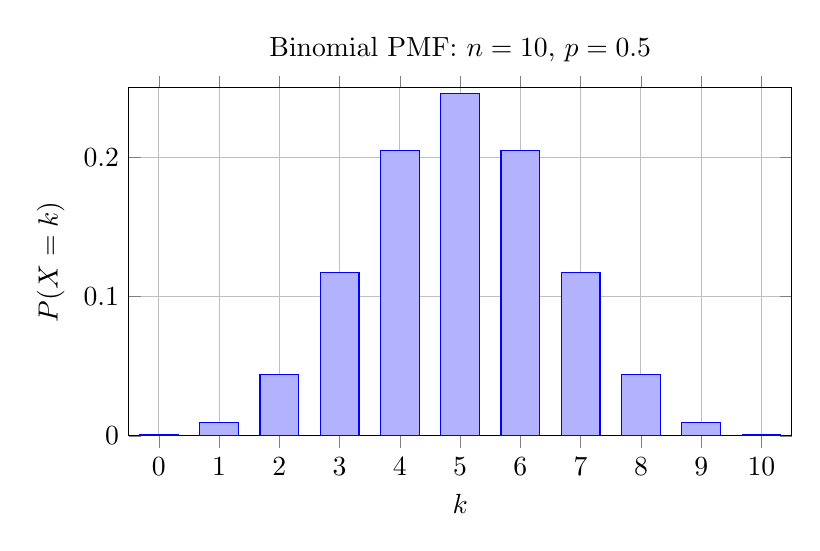
\begin{tikzpicture}
    \begin{axis}[
        ybar,
        bar width=14pt,
        ymin=0,
        ymax=0.25,
        xmin=-0.5,
        xmax=10.5,
        xtick={0,1,2,3,4,5,6,7,8,9,10},
        xlabel={$k$},
        ylabel={$P(X=k)$},
        title={Binomial PMF: $n=10$, $p=0.5$},
        width=10cm,
        height=6cm,
        grid=major
    ]
    \addplot+[blue,fill=blue!30] coordinates {
        (0,0.00098)
        (1,0.00977)
        (2,0.04395)
        (3,0.11719)
        (4,0.20508)
        (5,0.24609)
        (6,0.20508)
        (7,0.11719)
        (8,0.04395)
        (9,0.00977)
        (10,0.00098)
    };
    \end{axis}
\end{tikzpicture}
    \caption{PMF of the binomial distribution with $n=10$, $p=0.5$}
\end{figure}

Given that the binomial PDF is well-known, if we are able to map our experiment to a binomial distribution, 
we can use the properties of the binomial distribution to make predictions and calculate probabilities without needing to run additional experiments.

\paragraph{Bernoulli Random Variable}
The Bernoulli distribution is a special case of the binomial distribution where $n=1$.
It models a single trial with two possible outcomes: success (1) with probability $p$ and failure (0) with probability $1-p$.
The PMF of a Bernoulli random variable $X$ is:
\begin{equation}
    P(X=1) = p, \quad P(X=0) = 1-p
\end{equation}

\paragraph{Other PMFs Random Variables}
Other important discrete random variables include:
\begin{itemize}
    \item \textbf{Geometric}: Models the number of trials until the first success in a sequence of independent Bernoulli trials.
    \[ P(X=k) = (1-p)^{k-1} p \]
    \item \textbf{Negative Binomial}: Models the number of trials until a specified number of successes occurs.
    \[ P(X=k) = \binom{k-1}{r-1} p^r (1-p)^{k-r} \]
\end{itemize}

\subsection{Mastering Uncertainty}
In this section we will cover some important concepts and techniques to master uncertainty in experiments, 
which are essential for making informed decisions based on experimental results.

\subsubsection{Conditional Probability}
The \textbf{conditional probability} of an event $E$ given another event $F$ occurred is defined as:
\begin{equation}
    P(E|F) = \frac{P(E,F)}{P(F)}
\end{equation}
Which is the probability of both events $E$ and $F$ occurring, divided by the probability of event $F$ occurring.

\paragraph{Chain Rule}
The \textbf{chain rule}, also known as the product rule, allows us to express the joint probability of multiple events in terms of conditional probabilities:
\begin{equation}
    P(E,F) = P(E|F) P(F) = P(F|E) P(E)
\end{equation}

\paragraph{Generalized Chain Rule}
The \textbf{generalized chain rule} allows us to express the joint probability of multiple events in terms of conditional probabilities:
\begin{equation}
    P(E_1, E_2, ..., E_n) = P(E_1) P(E_2|E_1) P(E_3|E_1, E_2) ... P(E_n|E_1, E_2, ..., E_{n-1})
\end{equation}
If we have $P(F)=0$, then $P(E|F)$ is undefined, in other words, we cannot condition on an event that has zero probability of occurring.

\paragraph{Independent Case}
If $E$ and $F$ are \textbf{independent} events, then the occurrence of one does not affect the probability of the other. 
Applying the chain rule we have:
\begin{equation}
    P(E,F) = P(E|F)P(F) = P(E)P(F) 
\end{equation}

\subsubsection{Expectation}
The \textbf{expectation} is the summation of all possible values of a random variable, weighted by their probabilities.
It's also called mean, weighted average, or center of mass, and represents the average value we would expect from a random variable.
\begin{equation}
    E[X] = \sum_{x \in S} x P(X=x)
\end{equation}

We can also estimate the expectation from data using the sample mean:
\begin{equation}
    E[X] \approx \frac{1}{n} \sum_{i=1}^{n} x_i
\end{equation}
Where $x_i$ are the observed values of the random variable in our data, and $n$ is the number of observations.
Basically, we are calculating the average of the observed values, which is an estimate of the true expectation.

The expectation has several important \textbf{properties}:
\begin{itemize}
    \item \textbf{Linearity}: 
    \[
        E[aX + bY] = aE[X] + bE[Y]
    \]
    \item \textbf{Expectation of a sum}: 
        \[
            E[X + Y] = E[X] + E[Y]
        \]
    \item \textbf{Unconscious Statistician}: 
        \[
            E[g(X)] = \sum_{x \in S} g(x) P(X=x)
        \]
    \item \textbf{ Law of Total Expectation}: For any random variables $X$ and $Y$, we have:
        \[
            E[X] = \sum_{y \in S} E[X|Y=y] P(Y=y)
        \]
        Where $E[X|Y=y]$ is the conditional expectation of $X$ given $Y=y$.
\end{itemize}

\textbf{Foundational random variables} have specific expectations:
\begin{itemize}
    \item \textbf{Binomial random variable} $X \sim Bin(n, p)$, the expectation is:
    \[
        E[X] = \sum_{k=0}^{n} k p(X=k)
    \]
    Knowing that $p(X=k) = Bern(p)$, we can simplify the expectation to:
    \[
        E[X] = np
    \]
    \item \textbf{Bernoulli random variable} $X \sim Bern(p)$, the expectation is:
    \[
        E[X] = p
    \]
    \item \textbf{Geometric random variable} $X \sim Geo(p)$, the expectation is:
    \[    
        E[X] = \frac{1}{p}
    \]
\end{itemize}

However, the expectation is just a summary statistic, and it does not capture the variability of the random variable.
If not used carefully, it can be misleading, since it does not provide information about the spread or shape of the distribution.

\subsubsection{Variance}
The \textbf{variance} of a random variable measures the spread or variability of its distribution.
It is defined as the expected value of the squared deviation from the mean:
\begin{equation}
    Var(X) = E[(X - E[X])^2] = E[X^2] - (E[X])^2
\end{equation}
The variance is expressed in the square of the units of the random variable, which can make it less interpretable.
Then can be heavily influenced by outliers, as it squares the deviations from the mean.

Key properties of variance include:
\begin{itemize}
    \item \textbf{Non-negativity}: for any random variable $X$
        \[
            Var(X) \geq 0
        \]
    \item \textbf{Additivity for Independent Variables}: If $X$ and $Y$ are independent random variables
        \[
            Var(X + Y) = Var(X) + Var(Y)
        \].
    \item \textbf{Scaling}:for any constant $a$
        \[
            Var(aX) = a^2 Var(X)
        \]
    \item \textbf{Shift Invariance}: for any constant $c$
        \[
            Var(X + c) = Var(X)
        \]
    \item \textbf{Variance of a Sum}: For any random variables $X$ and $Y$
    \[
        Var(X + Y) = Var(X) + Var(Y) + 2Cov(X, Y)
    \]
    \item \textbf{Variance of Conditional Probability}: For any random variables $X$ and $Y$
    \[
        Var(X) = E[Var(X|Y)] + Var(E[X|Y])
    \]
\end{itemize}

\subsubsection{Law of Total Probability}
The \textbf{law of total probability} states that if $E_1, E_2, ..., E_n$ are mutually exclusive and exhaustive events, then for any event $F$, we have:
\begin{equation}
    P(F) = \sum_{i=1}^{n} P(F|E_i) P(E_i)
\end{equation}
This law allows us to calculate the probability of an event $F$ by considering all possible ways that $F$ can occur through the events $E_i$.
If we have only two events $E$ and $E^C$, then the law of total probability simplifies to:
\begin{equation}
    P(F) = P(F|E) P(E) + P(F|E^C) P(E^C)
\end{equation}

\subsubsection{Bayes' Theorem}
\textbf{Bayes' theorem} allows us to update our beliefs about the probability of an event $E$ given new evidence $F$:
\begin{equation}
    P(F|E) = \frac{P(E|F) P(F)}{P(E)}
\end{equation}
All the terms in Bayes' theorem have specific names:
\begin{itemize}
    \item $P(F|E)$ is the \textbf{posterior probability}, which is the updated probability of event $E$ after observing evidence $F$;
    \item $P(E|F)$ is the \textbf{likelihood}, which is the probability of observing evidence $F$ given that event $E$ is true;
    \item $P(F)$ is the \textbf{prior probability}, which is the initial belief about the probability of event $E$ before observing evidence $F$:
    \item $P(E)$ is the \textbf{marginal likelihood} or \textbf{evidence}, which is the total probability of observing evidence $F$ under all possible events.
\end{itemize}
What this theorem allows us to do is to update our beliefs about the probability of an event $E$ based on new evidence $F$, 
which is essential for making informed decisions in the face of uncertainty.

Apllying Bayes' theorem to the previous example of the AI Judge, we can define:
\begin{itemize}
    \item $E$: the observed outcomes of the judge's ratings (e.g., "good" or "not good");
    \item $F$: the underlying probability of the judge rating an output as "good". This clearly corresponds
    to the quality of the original AI system output, which is what we want to estimate;
    \item $P(F)$: our prior belief about the quality of the original AI system output. 
    This could be based on previous experiments (coming from the same domain), domain knowledge, or assumptions about the system's performance.
    It works as a rescaling factor that allows us to incorporate our prior beliefs into the analysis of the experiment.
    \item $P(E|F)$: the likelihood of observing the judge's ratings given a specific underlying probability of rating an output as "good".
\end{itemize}

\subsection{Beta Distribution}
When testing an AI system, we want to estimate the probability of success 
(e.g., the probability that the judge rates an output as "good") based on observed data. 
This could be done by either using the frequentist approach, simply giving the expected value of the binomial distribution, 
or by using the Bayesian approach, which allows us to give the full distribution of the probability of success, 
which is the \textbf{beta distribution}.

Given the previous example of the AI Judge, suppose that we want to compute the probability density that our original system output is "good" exactly 70\% of the time. 
Let the random variable $X \in [0, 1]$ represent the unknown probability of success, 
and let $E$ represent the evidence consisting of $s$ successes and $f$ failures. Using Bayes' Theorem:

\begin{equation}
    P(X = 0.7 | E) = \frac{P(E | X = 0.7) P(X = 0.7)}{P(E)}
\end{equation}

Given that the likelihood $P(E|X)$ follows a binomial distribution and supposing that we have a uniform prior distribution for $X$, we can derive the posterior distribution of $X$ as follows:

\begin{equation}
    P(X | E) = \frac{\binom{n}{s} X^s (1-X)^{n-s}}{P(E)}
\end{equation}
Where $n = s + f$ is the total number of trials (successes + failures).

Since $\binom{n}{s} \text{and} P(E)$ are constants with respect to $X$, we can write the posterior distribution as:
\begin{equation}
    P(X | E) \propto X^s (1-X)^{f}
\end{equation}
Which is the probability density function of a \textbf{beta distribution} with parameters $\alpha = s + 1$ and $\beta = f + 1$:

\paragraph{General Beta Distribution}
The general beta distribution is defined as:
\begin{equation}
    f_X(x) = \frac{x^{\alpha - 1} (1-x)^{\beta - 1}}{B(\alpha, \beta)} \quad \text{for } 0 < x < 1
\end{equation}
Where $\alpha$ and $\beta$ are the shape parameters of the distribution, and 
$B(\alpha, \beta)$ is the beta function, which serves as a normalization constant to ensure that the total probability integrates to 1.

\subsubsection{Experiment Design with Beta Distribution}
We are now going to see how to use the beta distribution to design experiments and make informed decisions based on the observed data.

\paragraph{Set parameters from data}
If we have observed $s$ successes and $f$ failures, we can set $\alpha = s + 1$ and $\beta = f + 1$ to get the posterior distribution of the probability of success.
This is helpful because it allows us to update our beliefs about the probability of success as we collect more data.

\paragraph{No prior Knowledge}
If we have no prior knowledge about the probability of success, we can set a uniform prior distribution for $X$, which corresponds to the $+1$ in the parameters of the beta distribution.
This represent a prior belief without any evidence, and allows us to incorporate the observed data in a way that reflects our updated beliefs about the probability of success.

\paragraph{Encoding Prior Knowledge}
If we have instead already experienced $s$ successes and $f$ failures previously, having a prior belief about the probability of success, we can set $\alpha = s + \alpha_0$ and $\beta = f + \beta_0$, 
where $\alpha_0$ and $\beta_0$ are the parameters of our prior distribution, and can be interpreted as imaginary successes and failures that we have observed before.

This creates a new posterior distribution that combines our prior belief with the observed data, allowing us to make more informed decisions.

\subsubsection{Expected Value and Variance}
The expected value of a beta distribution with parameters $\alpha$ and $\beta$ is given by:
\begin{equation}
    E[X] = \frac{\alpha}{\alpha + \beta}
\end{equation}
Where again $\alpha$ and $\beta$ are the parameters of the distribution, which can be interpreted respectively as the \textbf{number of successes} and the \textbf{number of failures} observed in the data.
This means that the expected value of the beta distribution can be interpreted as the estimated probability of success based on the observed data and our prior beliefs.

The variance of a beta distribution with parameters $\alpha$ and $\beta$ is given by:
\begin{equation}
    Var(X) = \frac{\alpha \beta}{(\alpha + \beta)^2 (\alpha + \beta + 1)}
\end{equation}
This variance captures the uncertainty in our estimate of the probability of success, and it decreases as we observe more data (i.e., as $\alpha$ and $\beta$ increase), 
reflecting the fact that our estimate becomes more precise as we gather more evidence.

\subsection{Adding Random Variables}
In some cases, we may want to add two random variables together, for example, to calculate the total number of successes in two independent experiments.
If $A$ and $B$ are two independent random variables, then the probability of the random variable $C$ representing the sum of $A$ and $B$ can be calculated through the law of total probability:
\begin{equation}
    P(C=k) = P(A+B=k) = \sum_{i=0}^{k} P(A=i) P(B=k-i)
\end{equation}
The basic idea is to consider all possible ways that the sum $C$ can equal $k$ by summing over all possible values of $A$ and $B$ that add up to $k$.

However, if $A$ and $B$ are not discrete random variables, we would need to use the convolution of their probability density functions to calculate the distribution of their sum.
\begin{equation}
    f_C(c) = \int_{-\infty}^{\infty} f_A(a) f_B(c - a) da
\end{equation}
The idea is to integrate over all possible values of $A$ and $B$ that sum up to $c$, weighted by their respective probability densities.

Sometimes, we variables are \textbf{i.i.d.} (independent and identically distributed), meaning they have the same:
\begin{itemize}
    \item All have the same distribution
    \item All have the same expectation
    \item All have the same variance
\end{itemize}
This simplifies the calculation of the distribution of their sum, since we can use the properties of the distribution to derive the distribution of the sum.

\subsubsection{Sum of Foundational Random Variables}
\begin{itemize}
    \item \textbf{Sum of Binomial Random Variables}: 
    \[
        X_1 \sim Bin(n_1, p), \quad X_2 \sim Bin(n_2, p) \implies X_1 + X_2 \sim Bin(n_1 + n_2, p)
    \]
    \item \textbf{Sum of Bernoulli Random Variables}:
    \[
        X_1 \sim Bern(p), \quad X_2 \sim Bern(p) \implies X_1 + X_2 \sim Bin(2, p)
    \]
    \item \textbf{Sum of Normal Random Variables}:
    \[
        X_1 \sim N(\mu_1, \sigma_1^2), \quad X_2 \sim N(\mu_2, \sigma_2^2) \implies X_1 + X_2 \sim N(\mu_1 + \mu_2, \sigma_1^2 + \sigma_2^2)
    \]
\end{itemize}

\subsubsection{Central Limit Theorem}
The \textbf{central limit theorem} states that the sum of a large number of independent and identically distributed random variables, each with finite mean and variance, will approximately follow a normal distribution, regardless of the original distribution of the variables.
\[
    \sum_{i=1}^{n} X_i \xrightarrow{d} N(n\mu, n\sigma^2) \quad \text{as } n \to \infty
\]
This implies that the sum of idd random variables is always \textbf{normally distributed}, where the $E[X_i] = \mu$ and $Var(X_i) = \sigma^2$ for all $i$.

\subsubsection{Sample Mean and Sample Variance}
Given a sample of $n$ independent and identically distributed random variables $X_1, X_2, ..., X_n$ with mean $\mu$ and variance $\sigma^2$, we can calculate the \textbf{sample mean} and \textbf{sample variance} as follows:
\begin{equation}
    \bar{X} = \frac{1}{n} \sum_{i=1}^{n} X_i
\end{equation}
\begin{equation}
    S^2 = \frac{1}{n-1} \sum_{i=1}^{n} (X_i - \bar{X})^2
\end{equation}
The sample mean $\bar{X}$ is an unbiased estimator of the population mean $\mu$, and the sample variance $S^2$ is an unbiased estimator of the population variance $\sigma^2$.

\subsection{Bootstraping}
Bootrapping allows us to know the distribution of a statistic (e.g., mean, variance) and calculate $p$-values without making assumptions about the underlying distribution of the data.

The idea is that we can approximate the real distribution of a statistic by sampling directly from the data we have, and calculating the statistic for each sample.
So we want to estimate the PMF of a statistic $T$ trough this algorithm:
\begin{enumerate}
    \item Repeat $B$ times:
    \begin{itemize}
        \item Draw a bootstrap sample of size $n$ from the original data
        \item Recalculate the statistic $T^*$ for the bootstrap sample
    \end{itemize}
\end{enumerate}
In order to enhance we can use \textbf{resampling with replacement}, which means that we can draw the same data point multiple times in the bootstrap sample, increasing the data available for estimation.
